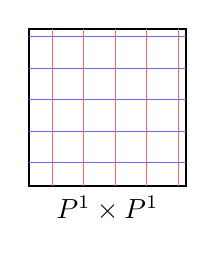
\begin{tikzpicture}[scale=2]
  % boundary square representing P^1 x P^1
  \draw[thick] (0,0) rectangle (1,1);

  % horizontal ruling (first P^1–factor)
  \foreach \y in {0.15,0.35,0.55,0.75,0.95}{
    \draw[blue!60] (0,\y) -- (1,\y);
  }

  % vertical ruling (second P^1–factor)
  \foreach \x in {0.15,0.35,0.55,0.75,0.95}{
    \draw[red!60] (\x,0) -- (\x,1);
  }

  % sample fiber labels
  % \node[blue!70!black, anchor=east] at (-0.02,0.75) {$\{p\}\times\mathbb{P}^1$};
  % \node[red!70!black, anchor=south] at (0.75,1.02) {$\mathbb{P}^1\times\{q\}$};

  % corner label
  \node[below] at (0.5,0) {$\mathbb{P}^1\times\mathbb{P}^1$};
\end{tikzpicture}